\subsection{Wederzijdse uitsluiting: hardwareondersteuning}

\subsubsection{Uitschakelen van interrupts}

Uniprocessor-systemen: concurrerende processen kunnen elkaar niet overlappen. Daarnaast zal een proces worden uitgevoerd tot het verzoekt om een dienst van het besturingssysteem of wanneer het onderbroken wordt. Het is daarom mogelijk om wederzijdse uitsluiting te garanderen door te voorkomen dat een proces onderbroken wordt. Dit werkt NIET in bij een multiprocessor-systeem.

\subsubsection{Speciale machine instructies}

\begin{figure}[htp]
    \centering
            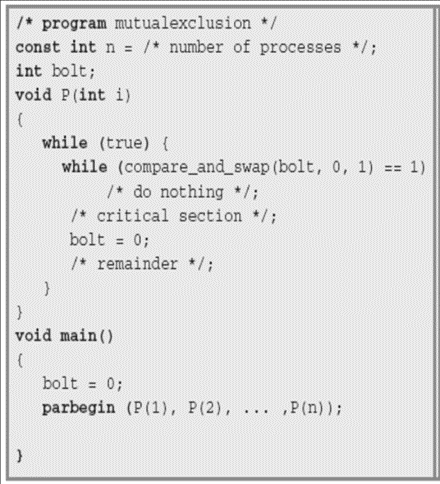
\includegraphics[width=4in]{img/compareandswap.png}
        \caption{Compare and Swap code voorbeeld}
    \label{fig:Compare and Swap code voorbeeld}
\end{figure}

\newpage

\subsubsubsection{Instructie exchange}
\begin{figure}[htp]
    \centering
            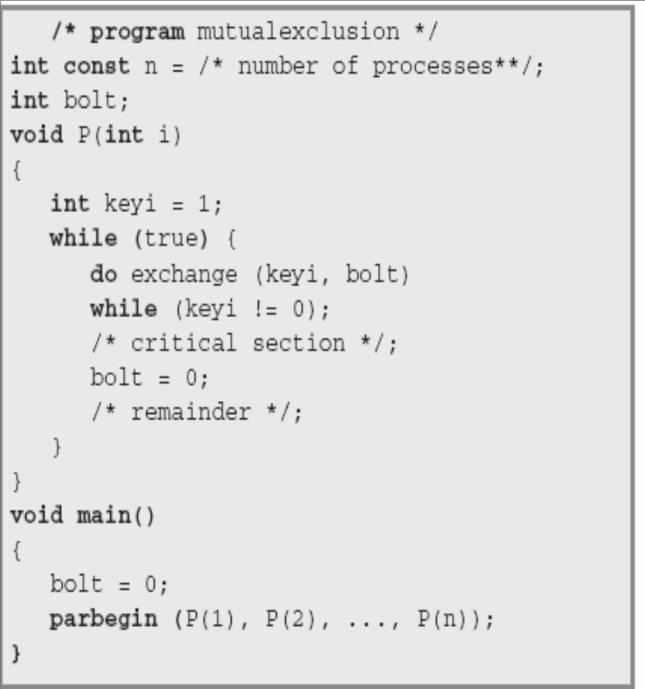
\includegraphics[width=4in]{img/instructieexchange.png}
        \caption{Voorbeeld van Instructie Exchange}
    \label{fig:Voorbeeld van Instructie Exchange}
\end{figure}


\subsubsubsection{Eigenschappen van de benadering met machine-instructies}

\textbf{Voordelen van het werken met machine-instructies:}

\begin{itemize}
\item Toepasbaar op alle processen op een machine met 1 processor en op alle processen op een systeem van multiprocessing die het hoofdgeheugen delen.
\item Dit is eenvoudig en makkelijk te controleren.
\item Kan worden gebruikt voor het ondersteunen van meerdere kritieke secties waarbij elke kritieke sectie zijn eigen variabele kan hebben.
\end{itemize}

\textbf{Nadelen van het werken met machine-instructies:}

\begin{itemize}
\item Busy-waiting: proces blijft processortijd verbruiken terwijl het niets nuttig aan het doen is.
\item Starvation kan nog steeds: aangezien het willekeurig is welk proces een proces opvolgt dat uit zijn kritieke sectie komt en als er meerdere processen zijn die 'busy waiting' zijn, dan kan het zijn dat een proces zeer lang in de wachtrij staat.
\item Deadlock: P1 gaat in kritieke sectie maar wordt onderbroken door P2 dat een hogere prioriteit heeft, echter, om te voltooien heeft P2 dezelfde bron nodig als P1 maar die is geblokkeerd door P2 en P1 wacht op de voltooiing van P2... (dan maakt het niet uit of er even een ander proces wordt geactiveerd want de clue is dat deze twee processen niet verder kunnen, tenzij het OS P2 plots een lagere prioriteit geeft dan P1 waardoor P1 weer actief kan worden...).
\end{itemize}
